
\section{Common neighbor rule}


In their study, Perin et al.\ follow their report of increased edge
counts in neuron clusters with the observation of a \enquote{common
  neighbor rule}\index{common neighbor rule}: Relying once again on
their data in the rat's somatsensory cortex, Perin et al.\ find that
not only do neuron pairs with a high number of common neighbor count
\marginpar{common neighbor rule as underlying principle?} appear
significantly more often than expected, but also that such pairs
display a higher probability of being connected. In fact, the
relationship between pair connectivity and number of common neighbors
appears to be linear. Perin et al.\ also report that this effect is
most pronounced when only considering common in-neighbors, that is
other neurons that are projecting to both neurons in the pair.

Here we also investigate our networks for the existence of such a
common neighbor relationship. Simultaneously recording connection
probabilities and the number of common neighbors between pairs of
neurons, we find inherent dependencies between the two quantities in
all network types (\autoref{fig:cm_rule}). 

\vspace{-0.25cm}
\begin{figure}[H]
  \centering
  \makebox{%
    \begin{overpic}[width=0.5\textwidth]{%
         plots/5841710e_in.pdf}
      \put(21,56.6){\small\textbf{A}}
    \end{overpic}
    \hfill
    \begin{overpic}[width=0.5\textwidth]{%
        plots/5841710e_out.pdf}
      \put(21,56.6){\small\textbf{B}}
    \end{overpic}
  }%
  \vfill
  \vspace{0.11cm}
  \makebox{%
    \begin{overpic}[width=0.5\textwidth]{%
         plots/5841710e_all.pdf}
       \put(21,56.6){\small\textbf{C}}
    \end{overpic}
    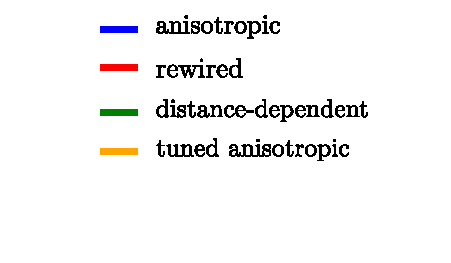
\includegraphics[width=0.5\textwidth]{%
      img/common_neighbor_legend.pdf}
  }
  \vfill
  \vspace{0.11cm}
  \makebox{%
    \begin{overpic}[width=0.5\textwidth]{%
         plots/5841710e_in_k.pdf}
      \put(20.5,57.5){\small\textbf{D}}
    \end{overpic}
    \hfill
    \begin{overpic}[width=0.5\textwidth]{%
        plots/5841710e_out_k.pdf}
      \put(20.5,57.5){\small\textbf{E}}
    \end{overpic}
  }%
  \captionsetup{skip=7pt}
  \caption{\textbf{Common neighbor rules in the different network
      types} Showing the dependency of connection probability on the
    number of shared neighbors for random neuron pairs, characteristic
    curves for the network types (see legend) arises. High error
    margins (errorbars SEM) for small number of common neighbors in
    distance-dependent networks is induced by vanishingly low occurrence
    of a small common neighbor count. (\smtcite{5841710e})}
  \label{fig:cm_rule}
\end{figure}


Analyzing the results, we immediately note the sharp difference
between in- and out-neighbors in their effect on connection
probabilities in anisotropic networks, as well as in rewired
networks. Only in distance-dependent networks it appears that in- and
out-neighbors can be considered equivalent in their influence on
connection probabilities (\autoref{fig:cm_rule} A-B). Furthermore,
while the distribution of the number of common neighbors is consistent
in distance-dependent networks, the other network types display a
characteristic distribution of common out-neighbors
(\autoref{fig:cm_rule} D-E). While the latter observation clearly also
relates to the differences in out-degree distributions found in
Section~\ref{sec:degree_distribution}, finding differences between
common inputs and outputs in neuron pairs is consistent with the
observations of Perin et al., who report a significant difference in
effect of the common neighbor rule. In trying to model the inherently
asymmetric axonal-dendritic connections between pyramidal cells in
cortical circuits with the anisotropic networks, finding such
disparity is not only expected but gives the model further validity as
an approach to obtain network connectivity going beyond the
distance-dependent archetype, which here fails to produce diverging
connectivity statistics for in- and outputs.
% Intertrepation: Connectivity
% in cortex asymmetric: synapse cortex
% and with Perin result in vs out

Both for in- and out-neighbors, we find characteristic curves
describing their influence on connection probabilities. The
in-neighbor profiles split into two categories: While networks with
anisotropy in connectivity (blue, orange) display a constant increase,
distance-dependent network types (red, green) \marginpar{anisotropy
  induces characteristic common neighbor rule} show a sigmoidal shared
input-connection probability curve (\autoref{fig:cm_rule} A).  We thus
find a strong influence of anisotropy on the shared input
relationship, inducing a common neighbor rule characteristically
different from isotropic, distance-depen\-dent networks.

Does this anisotropy-induced rule reflect the findings in cortical
networks?  Perin et al.\ report a linear common neighbor relationship,
finding a stronger effect when considering only in-neighbors. Imposing
the common neighbor rule on \textit{in silico} networks reflecting a
distance-dependency as determined \textit{in vivo}, Perin et al.\ were
then able to reproduce the observed overrepresentation of high edge
counts in neuron clusters, identifying the common neighbor effect as
an underlying connection principle inducing increased high edge counts
in clusters comparable to the profiles shown in
\autoref{fig:perin6to12}. Showing not only the presence of such an
edge count \marginpar{anisotropy as underlying connection principle!}
overrepresentation in anisotropic networks, but also finding that only
networks featuring anisotropy display an approximately linear
relationship between common inputs and connection probability, we
identify anisotropy in connectivity as a candidate for an underlying
connection principle motivated from neuronal morphology, to induce a
common neighbor rule, that may be at the heart of many of the
non-random connectivity statistics observed in local cortical
networks.

Extending the analysis of shared inputs in the different network
types, we further observe that anisotropy affects the number of common
in-neighbors typically observed itself (\autoref{fig:cm_rule} D). We
specifically find that increases anisotropy in connectivity induces an
increased variance in the distribution of common inputs of a random
neuron pair \autoref{fig:common_input_rew}). Such increased variance
may provide an important advantage in the processing of information,
allowing a heightened functional specificity in the network, where
many neurons do not share many common inputs, enabling a high variety
of functionality, and where few neuron pairs have a high number of
shared inputs, strengthening their correlation and thus their capacity
to relay related information.


\begin{figure}[H]
  \centering
  \makebox{%
    \begin{overpic}[width=0.493\textwidth]{%
        plots/5841710e_in_k_tanfitrew.pdf}
      \put(87.5,58.2){\small\textbf{A}}
    \end{overpic}
    \hfill
    \begin{overpic}[width=0.5\textwidth]{%
        plots/ffcefe9b.pdf}
      \put(89,58.2){\small\textbf{B}}
    \end{overpic}
  }%
  \captionsetup{skip=7pt}
  \caption{\textbf{Anisotropy increases variance of common input
      distribution} Recording common in-neighbor counts for random
    neuron pairs in tuned anisotropic networks and their rewired
    versions reveals increased variance in networks with a high degree
    of anisotropy. \textbf{A)} Common in-neighbor distribution for
    original tuned anisotropic networks ($\eta = 0$, blue) and rewired
    versions with $\nicefrac{1}{4}$ of all edges rewired ($\eta =
    0.25$, red) and completely rewired ($\eta =1 $, green).
    (\smtcite{5841710e}) \textbf{B)} Variance of the common
    in-neighbor distributions declines with increasing rewiring factor
    $\eta$; highest variance is found in networks with the highest
    degree of anisotropy ($\eta = 0$). Errorbars SEM. (\smtcite{ffcefe9b})}
  \label{fig:common_input_rew}
\end{figure}


%%% Local Variables: 
%%% mode: latex
%%% TeX-master: "../dplths_document"
%%% End: 
